% Chapter 1. The three budgets, and the fact that they trade against each other.
\documentclass[tikz,border=6pt]{standalone}
% Shared look for every TikZ figure in the book.
% Colours match book/preamble.tex exactly. Change both or neither.

\usepackage{tikz}
\usepackage{xcolor}
\usepackage{amsmath}
\IfFileExists{libertinus.sty}{\usepackage[mono=false]{libertinus}}{}
\IfFileExists{inconsolata.sty}{\usepackage[varqu,varl,scaled=0.95]{inconsolata}}{}

\usetikzlibrary{
  arrows.meta, positioning, calc, fit, backgrounds, shapes.geometric,
  shapes.misc, decorations.pathreplacing, decorations.pathmorphing,
  patterns, chains, matrix, shadows.blur
}

\definecolor{ink}{HTML}{15181D}
\definecolor{muted}{HTML}{5B6472}
\definecolor{rule}{HTML}{C9CED6}
\definecolor{wash}{HTML}{F4F5F7}
\definecolor{accent}{HTML}{0F5C8C}
\definecolor{accentsoft}{HTML}{E7F0F6}
\definecolor{warm}{HTML}{B4531A}
\definecolor{warmsoft}{HTML}{FBF0E7}
\definecolor{good}{HTML}{2C6E49}
\definecolor{goodsoft}{HTML}{E9F2EC}
\definecolor{danger}{HTML}{9B2226}
\definecolor{dangersoft}{HTML}{FAECEC}

\tikzset{
  font=\sffamily\small,
  >={Stealth[length=5pt, width=4pt]},
  %
  box/.style={
    draw=rule, line width=0.8pt, fill=wash, rounded corners=2pt,
    inner sep=7pt, align=center, text=ink, minimum height=9mm,
  },
  boxa/.style={box, draw=accent, fill=accentsoft},
  boxg/.style={box, draw=good,   fill=goodsoft},
  boxw/.style={box, draw=warm,   fill=warmsoft},
  boxd/.style={box, draw=danger, fill=dangersoft},
  %
  lane/.style={draw=rule, line width=0.7pt, fill=white, rounded corners=2pt,
               inner sep=6pt, align=center, minimum width=26mm},
  %
  flow/.style={draw=accent, line width=1.0pt, ->},
  flowback/.style={flow, densely dashed},
  flowmuted/.style={draw=muted, line width=0.8pt, ->},
  lifeline/.style={draw=rule, line width=0.7pt, densely dotted},
  %
  lbl/.style={font=\sffamily\scriptsize, text=muted, inner sep=2pt},
  lblink/.style={font=\sffamily\scriptsize, text=ink, inner sep=2pt},
  tag/.style={font=\ttfamily\scriptsize, text=accent, inner sep=2pt,
              fill=white, inner xsep=3pt},
  note/.style={font=\sffamily\scriptsize\itshape, text=muted, align=left},
  %
  band/.style={draw=none, rounded corners=1pt},
  tick/.style={draw=muted, line width=0.6pt},
}

% A horizontal timeline bar segment: \barseg{x0}{x1}{y}{colour}{label}
\newcommand{\barseg}[5]{%
  \fill[#4, rounded corners=1pt] (#1,#3-0.16) rectangle (#2,#3+0.16);
  \node[lbl, text=white, font=\sffamily\scriptsize\bfseries]
       at ({(#1+#2)/2},#3) {#5};
}

\begin{document}
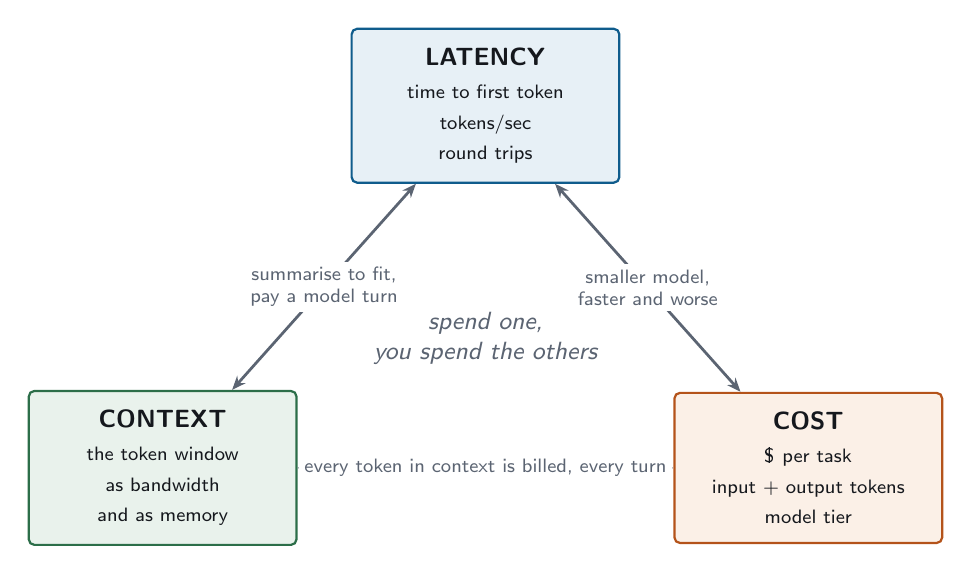
\begin{tikzpicture}[x=1cm, y=1cm]

  \def\R{2.55}

  % --- the three budgets, as a triangle of tradeoffs ---------------------
  \node[boxa, minimum width=34mm, align=center] (lat) at (0,3.1)
    {\textbf{LATENCY}\\[1pt]\scriptsize time to first token\\\scriptsize tokens/sec\\\scriptsize round trips};

  \node[boxg, minimum width=34mm, align=center] (ctx) at (-4.1,-1.5)
    {\textbf{CONTEXT}\\[1pt]\scriptsize the token window\\\scriptsize as bandwidth\\\scriptsize and as memory};

  \node[boxw, minimum width=34mm, align=center] (cost) at (4.1,-1.5)
    {\textbf{COST}\\[1pt]\scriptsize \$ per task\\\scriptsize input + output tokens\\\scriptsize model tier};

  % --- the tradeoff edges ------------------------------------------------
  \draw[<->, draw=muted, line width=1pt] (lat) -- node[lbl, fill=white, inner sep=2pt,
        align=center, pos=0.5] {summarise to fit,\\pay a model turn} (ctx);
  \draw[<->, draw=muted, line width=1pt] (lat) -- node[lbl, fill=white, inner sep=2pt,
        align=center, pos=0.5] {smaller model,\\faster and worse} (cost);
  \draw[<->, draw=muted, line width=1pt] (ctx) -- node[lbl, fill=white, inner sep=2pt,
        align=center, pos=0.5] {every token in context is billed, every turn} (cost);

  % --- the centre --------------------------------------------------------
  \node[align=center, font=\sffamily\small\itshape, text=muted] at (0,0.15)
    {spend one,\\you spend the others};

\end{tikzpicture}
\end{document}
